\subsection{Décomposition en sous-domaines}
Le parallélisme dans la partie solveur linéaire du code peut être obtenu de deux façons différentes.
%
Jusqu'à maintenant, nous avons étudié le parallélisme avec des paradigmes de parallélisation en mémoire partagée, mais on peut aussi utiliser une parallélisation par passage de messages.
%
En pratique, nous allons utiliser les deux types de parallélisme pour exploiter au mieux les grappes de serveurs.
%
Mais on pourrait imaginer n'utiliser que le paradigme par passage de messages.
%
Dans ce cas, on change le préconditionneur et donc le résultat.
%
On va utiliser la décomposition de domaine pour distribuer le travail entre les différents processus.
%
Chaque processus traitera un domaine qui correspond un sous-ensemble des cellules du réservoir.
%
Le nouveau préconditionneur sera toujours une factorisation ILU mais seulement sur les sous ensemble de cellules.
%
Ici le parallélisme est idéal, chaque processus pourra exécuter une factorisation ILU parallèlement aux autres processus.
%
Malgré ce parallélisme, nous n'obtenons pas une accélération parfaite (Fig.~\ref{fig:res_facto_mpi}).
%
C'est un problème récurrent quand on fait de l'algèbre linéaire.
%
Si on compare les accélérations obtenues avec celles obtenues avec l'agrégation de tâches on peut voir des résultats légèrement meilleurs mais il ne faut pas oublier que le résultat numérique est moins bon et ce dernier critère est très dur à évaluer.
%
En effet, un résultat numérique moins bon peut engendrer plus d'itérations dans le solveur linéaire et donc consommer plus de temps.


%   (-_-)   %
\begin{figure}[t!]
  \centering
  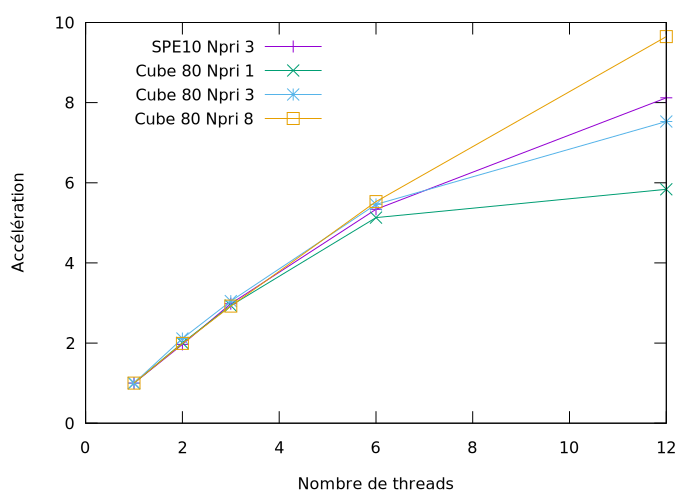
\includegraphics[width=0.7\textwidth]{res_facto_mpi}
  \caption{Performance de la factorisation sur 12 coeurs en utilisant la décomposition de domaine.}
  \label{fig:res_facto_mpi}
\end{figure}

%   (-_-)   %
\begin{figure}[t!]
  \centering
  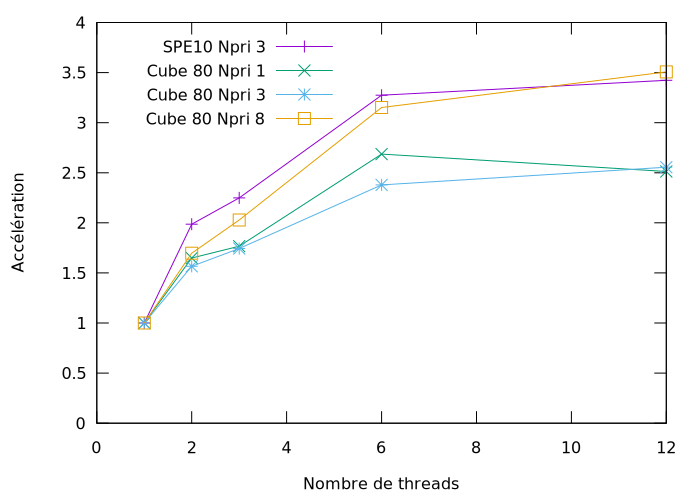
\includegraphics[width=0.7\textwidth]{res_trsv_mpi}
  \caption{Performance de la résolution triangulaire sur 12 coeurs en utilisant la décomposition de domaine.}
  \label{fig:res_trsv_mpi}
\end{figure}


La bande passante est au mieux de 16~Go/s, avec les threads nous utilisons 12~Go/s de bande passante locale dont 5~Go/s de bande passante distante.
%
Cette bande passante distante est le résultat des effets NUMA.
%
Dans le cas des processus MPI, chaque processus a son propre espace mémoire et la localité des données est assurée.
%
Mais dans le cas des threads, l'espace mémoire est partagée entre deux bancs mémoires et si les accès mémoires ne sont pas optimisés, il y aura des transferts entre les bancs NUMA.
%
Ces transferts auront pour effet d'augmenter la latence des accès mémoires et de réduire le CPI\footnote{Clock Per Instruction}, ici on a un CPI de 0,75 pour la version MPI contre 1,08 pour la version threadé.
%
L'explication de la différence de performance entre ces deux versions se situe au niveau de la mémoire, on est limité par la bande passante.

%% +-----------------------------+----------+----------+MPI12
%% |           Metric            |  core 0  |  core 6  |
%% +-----------------------------+----------+----------+
%% |     Runtime (RDTSC) [s]     | 115.248  | 115.248  |
%% |    Runtime unhalted [s]     | 124.295  | 124.907  |
%% |         Clock [MHz]         | 3050.46  | 3053.54  |
%% |             CPI             | 0.751758 | 0.753133 |
%% | Memory bandwidth [MBytes/s] | 15905.1  | 15835.6  |
%% | Memory data volume [GBytes] | 1833.04  | 1825.02  |
%% |  Remote Read BW [MBytes/s]  | 10.3343  | 23.2978  |
%% | Remote Write BW [MBytes/s]  | 0.913861 | 1.61113  |
%% |    Remote BW [MBytes/s]     | 11.2482  | 24.9089  |
%% +-----------------------------+----------+----------+


%% +-----------------------------+----------+----------+MPI6(2*3)
%% |           Metric            |  core 0  |  core 6  |
%% +-----------------------------+----------+----------+
%% |     Runtime (RDTSC) [s]     | 155.807  | 155.807  |
%% |    Runtime unhalted [s]     | 168.391  | 168.976  |
%% |         Clock [MHz]         | 3055.54  | 3055.33  |
%% |             CPI             | 0.544832 | 0.510243 |
%% | Memory bandwidth [MBytes/s] |  11664   | 11561.2  |
%% | Memory data volume [GBytes] | 1817.34  | 1801.31  |
%% |  Remote Read BW [MBytes/s]  | 6.52392  | 31.9625  |
%% | Remote Write BW [MBytes/s]  | 0.532458 | 1.44266  |
%% |    Remote BW [MBytes/s]     | 7.05638  | 33.4051  |
%% +-----------------------------+----------+----------+

%% +-----------------------------+----------+----------+MPI6(1*6)
%% |           Metric            |  core 0  |  core 6  |
%% +-----------------------------+----------+----------+
%% |     Runtime (RDTSC) [s]     | 226.632  | 226.632  |
%% |    Runtime unhalted [s]     | 0.422044 | 245.002  |
%% |         Clock [MHz]         | 2518.14  | 3046.49  |
%% |             CPI             | 1.14334  | 0.728566 |
%% | Memory bandwidth [MBytes/s] | 13.2691  | 16633.6  |
%% | Memory data volume [GBytes] |  3.0072  | 3769.69  |
%% |  Remote Read BW [MBytes/s]  |  5.9309  | 1.91099  |
%% | Remote Write BW [MBytes/s]  | 0.362203 | 0.167456 |
%% |    Remote BW [MBytes/s]     |  6.2931  | 2.07845  |
%% +-----------------------------+----------+----------+


%% +-----------------------------+---------+---------+THREAD_NO_AGG
%% |           Metric            | core 0  | core 6  |
%% +-----------------------------+---------+---------+
%% |     Runtime (RDTSC) [s]     | 1761.37 | 1761.37 |
%% |    Runtime unhalted [s]     | 1679.57 | 1638.75 |
%% |         Clock [MHz]         | 2845.78 | 2792.27 |
%% |             CPI             | 5.57235 | 5.68339 |
%% | Memory bandwidth [MBytes/s] | 5263.52 | 3232.11 |
%% | Memory data volume [GBytes] | 9271.02 | 5692.95 |
%% |  Remote Read BW [MBytes/s]  | 1919.77 | 1341.83 |
%% | Remote Write BW [MBytes/s]  | 170.677 | 112.472 |
%% |    Remote BW [MBytes/s]     | 2090.45 | 1454.3  |
%% +-----------------------------+---------+---------+


%% +-----------------------------+---------+---------+THREAD_AGG_3
%% |           Metric            | core 0  | core 6  |
%% +-----------------------------+---------+---------+
%% |     Runtime (RDTSC) [s]     | 183.336 | 183.336 |
%% |    Runtime unhalted [s]     | 170.046 | 179.213 |
%% |         Clock [MHz]         | 2834.78 | 2872.02 |
%% |             CPI             | 1.08397 | 1.07228 |
%% | Memory bandwidth [MBytes/s] |  11668  |  12351  |
%% | Memory data volume [GBytes] | 2139.16 | 2264.38 |
%% |  Remote Read BW [MBytes/s]  | 5103.69 | 5256.16 |
%% | Remote Write BW [MBytes/s]  | 287.67  | 277.104 |
%% |    Remote BW [MBytes/s]     | 5391.36 | 5533.27 |
%% +-----------------------------+---------+---------+
